\documentclass[11pt]{article}
\usepackage[T1]{fontenc}
\usepackage[utf8]{inputenc}
\usepackage{lmodern}
\usepackage[margin=1in]{geometry}
\usepackage{amsmath,amssymb,amsthm,mathtools,mathrsfs}
\usepackage{microtype,booktabs,array,xcolor,xurl,graphicx,tikz}
\usepackage[colorlinks=true,linkcolor=blue!50!black,citecolor=blue!50!black,urlcolor=blue!50!black]{hyperref}
\hypersetup{pdftitle={Sharp binary-information contraction on the discrete cube},pdfauthor={OpenAI},pdfsubject={Binary information, entropy production, and cube noise}}
\newtheorem{theorem}{Theorem}[section]
\newtheorem{proposition}[theorem]{Proposition}
\newtheorem{lemma}[theorem]{Lemma}
\newtheorem{corollary}[theorem]{Corollary}
\theoremstyle{definition}
\newtheorem{definition}[theorem]{Definition}
\theoremstyle{remark}
\newtheorem{remark}[theorem]{Remark}
\newcommand{\E}{\mathbb E}
\DeclareMathOperator{\Var}{Var}
\DeclareMathOperator{\Cov}{Cov}
\numberwithin{equation}{section}
\setlength{\emergencystretch}{2em}
\allowdisplaybreaks[1]
\title{Sharp binary-information contraction\\on the discrete cube}
\author{OpenAI}
\date{September 24, 2026}
\begin{document}
\maketitle
\begin{abstract}
We prove sharp contraction of the information carried by a binary channel
under independent symmetric noise on a uniform discrete cube. At fixed
initial information, a noisy coordinate retains the most information.
The Boolean specialization resolves the Courtade--Kumar conjecture and
gives an output-entropy refinement. We also establish a stronger
mean-dependent entropy-production bound. The proof combines an explicit
three-point optimizer for the local joining problem, two entropy
capacities, and a common-output thinning inequality, followed by dimension
induction and integration along the noise semigroup.
\end{abstract}

\section{The contraction theorem and its mechanism}
\label{main:section}

A one-bit summary of independent fair bits can be chosen before those
bits pass through independent binary symmetric channels. Which summary
retains the most information about the noisy observation? Kumar and
Courtade formulated the conjecture that a single input coordinate is
optimal at every noise level and in every dimension
\cite{KumarCourtade2013,CourtadeKumar2014}. We prove a sharp comparison
for arbitrary randomized binary summaries, together with a
mean-dependent bound on their instantaneous information loss.

Let $\Omega_n=\{-1,1\}^n$ carry uniform measure. All information
is measured with natural logarithms. For $r\in[-1,1]$, define
\[
 L=\log2,\qquad
 H(r)=-\frac{1+r}{2}\log\frac{1+r}{2}
      -\frac{1-r}{2}\log\frac{1-r}{2},\qquad \psi(r)=L-H(r),
\]
with $0\log0=0$. Thus $H(r)$ is the entropy of a sign of mean $r$.
For a soft binary channel $u:\Omega_n\to[-1,1]$, define
\[
 I(u)=H(\E u)-\E H(u)=\E\psi(u)-\psi(\E u).
\]
Let $X$ be uniform on $\Omega_n$. If an auxiliary sign $U$ has conditional mean
$\E[U\mid X]=u(X)$, then $I(u)=I(U;X)$.  For
$-1\le\rho\le1$, let $Y_i=X_iZ_i$, where the signs $Z_i$
are independent of $(X,U)$ and each other, with $\E Z_i=\rho$.
The noise operator is $T_\rho u(y)=\E[u(X)\mid Y=y]$.
Thus $\E[U\mid Y]=T_\rho u(Y)$ and $I(T_\rho u)=I(U;Y)$.

\begin{theorem}[Sharp soft-channel contraction]
\label{main:soft}
For every finite $n\ge0$, every $u:\Omega_n\to[-1,1]$, and
$-1\le\rho\le1$,
\begin{equation}
 I(T_\rho u)
 \le\psi\!\left(|\rho|\,\psi^{-1}(I(u))\right).
 \label{main:interpolation}
\end{equation}
The inverse is the nonnegative increasing branch on $[0,L]$.
For $n\ge1$, every soft coordinate $u(x)=a x_i$, $|a|\le1$,
attains equality.
\end{theorem}

The parameter $\psi^{-1}(I(u))$ is the amplitude of a fair soft
coordinate with the same information as $u$.  The theorem says that
this effective amplitude contracts at least as fast as a coordinate.
Sharpness concerns all soft channels at a given initial information;
it does not assert that every biased Boolean source attains the bound.

\begin{corollary}[The Boolean bound with output bias]
\label{main:ck}
For every finite $n\ge0$, $\rho\in[-1,1]$, and
$f:\Omega_n\to\{-1,1\}$, put
$m=\E f$ and $r_m=\psi^{-1}(H(m))$.  Then
\begin{equation}
 I(f(X);Y)\le\psi(|\rho|r_m)\le\psi(|\rho|).
 \label{main:bound}
\end{equation}
For $n\ge1$, signed coordinate functions attain the bound at $m=0$.
If $0<|m|<1$ and $0<|\rho|\le1$, the refined upper curve is
strictly below the universal curve $\psi(|\rho|)$.
\end{corollary}

For noise crossover probability $\varepsilon\in[0,1/2]$, one has
$\rho=1-2\varepsilon$. Writing
$h_2(p)=-p\log_2p-(1-p)\log_2(1-p)$, the universal bound in bits is
\[
 I_2(f(X);Y)\le\frac{\psi(\rho)}{L}=1-h_2(\varepsilon).
\]
This is the Courtade--Kumar conjecture. The refinement uses the actual
entropy of the Boolean output, while the input distribution remains uniform.

\subsection{Prior work and related results}

Ordentlich, Shayevitz, and Weinstein
\cite{OrdentlichShayevitzWeinstein2016} obtained asymptotically sharp
high-noise bounds for balanced Boolean functions. Samorodnitsky
\cite{Samorodnitsky2016} proved the conjecture for all
Boolean functions in a dimension-independent high-noise range.
Yu's work on $\Phi$-stability and local optimality
\cite{Yu2023,Yu2026} enlarged the proved range for balanced functions;
the latter gives $0\le\rho\le0.914$ by a computer-assisted argument.
Javanmard and Woodruff \cite{JavanmardWoodruff2026} extended
Courtade and Kumar's coordinatewise sum bound
\cite[Theorem~1]{CourtadeKumar2014} from balanced functions to
arbitrary output bias and refined high-noise entropy estimates.

Several nearby formulations clarify the role of the full noisy vector.
Pichler, Piantanida, and Matz \cite{PichlerPiantanidaMatz2018} proved
coordinate optimality when the observation is also reduced to one
Boolean output. At fixed output mean, Li and M\'edard
\cite{LiMedard2021} identified lexicographic optimizers at sufficiently
low noise and related high-noise optimizers to first-level Fourier
weight, in dimension-dependent ranges. Barnes and \"Ozg\"ur
\cite{BarnesOzgur2020} proved the equivalence of the balanced conjecture
and a symmetrized Li--M\'edard moment inequality.
Kindler, O'Donnell, and Witmer \cite{KindlerODonnellWitmer2016}
proved fixed-mean Gaussian and spherical analogues. These fixed-mean
questions are distinct from attainability of the refined upper curve
in Corollary~\ref{main:ck}.

Chen, Gohari, and Nair \cite{ChenGohariNair2025} developed the
differential approach that we use: prove a local entropy-production
inequality, lift it by induction on the cube dimension, and integrate
along the noise semigroup. Their approach builds on the auxiliary
receiver method of Gohari and Nair \cite{GohariNair2022}. The
August 2026 revision of Chen--Gohari--Nair disproves one proposed auxiliary inequality
\cite[Appendix~B]{ChenGohariNair2025}; the local comparisons below
are proved directly. Their symmetric optimizer is a predecessor of
our arbitrary-mean joining problem, as explained in
Section~\ref{canonical:section}.

Recent preprints announce proofs of the Courtade--Kumar conjecture by
several routes. Chen, Gohari, Javanmard, Lin, Mirrokni, Nair, and
Woodruff~\cite{ChenEtAl2026CK} use a computer-assisted Bellman inequality;
Ky and Tran~\cite{KyTran2026CK} develop entropy-production and spectral
estimates with computer-assisted verification;
Mahdavifar and Beirami~\cite{MahdavifarBeirami2026CK} use
entropy flow, Fourier analysis, and bounds for pivotal sets; and
Kramer and Saglam~\cite{KramerSaglam2026} prove a finite-noise
bound that retains the Boolean output bias.
The overlap with the first work extends beyond the Boolean conjecture:
its Lemma~9.2 applies to arbitrary binary channels, and retaining the
initial information when integrating its production bound gives
Theorem~\ref{main:soft} and Corollary~\ref{main:ck}.
Our proof solves the joining problem with a common entropy budget and
uses two capacities and common-output thinning. It also proves the additional
mean-dependent production estimate in
Theorem~\ref{upgrade:production}; we compare the two production
profiles in Section~\ref{flow:comparison}.

\subsection{From information loss to a local joining inequality}

For an interior soft field $g:\Omega_n\to(-1,1)$, put
\begin{equation}
 m=\E g,\qquad e=\E H(g),\qquad I(g)=H(m)-e,
 \qquad D(g)=\E[V(g)Ng],
 \label{main:functionals}
\end{equation}
where $V(r)=\operatorname{atanh}r$ and
\[
 N=\frac12\sum_{i=1}^n(\mathrm{Id}-\mathrm{flip}_i),
 \qquad P_t=T_{e^{-t}}=e^{-tN}.
\]
Here $\mathrm{flip}_i$ flips coordinate $i$. Mean conservation and
finite-dimensional differentiation give
\begin{equation}
 \frac{d}{dt}I(P_tg)=-D(P_tg).
 \label{main:flow-identity}
\end{equation}
The production of a soft coordinate $g(x)=r x_i$ is $rV(r)$.
We therefore define its rate by
$F(\psi(r))=rV(r)$ for $0\le r<1$ and seek the inequality
$D(g)\ge F(I(g))$. Once this is proved,
$r_t=\psi^{-1}(I(P_tg))$ satisfies $r_t'\le-r_t$ whenever
$I(P_tg)>0$. Integrating gives Theorem~\ref{main:soft};
Section~\ref{flow:section} treats zero information and boundary-valued
inputs.

The local-to-global program is due to
Chen--Gohari--Nair \cite[Definition~1 and Theorem~2]{ChenGohariNair2025}.
To see the required local comparison, split the cube along one
coordinate into fields $g_+,g_-$ on $\Omega_{n-1}$. Their productions
satisfy the exact identity
\begin{equation}
 D(g)=\frac{D(g_+)+D(g_-)}2+\E c(g_+,g_-),\qquad
 c(a,b)=\frac{a-b}{4}\{V(a)-V(b)\},
 \label{main:energy-split}
\end{equation}
where the last expectation is over the remaining coordinates.
Write $m_\pm=\E g_\pm$ and $I_\pm=I(g_\pm)$.
For a profile with $\Phi_m(0)=0$, the required induction step is that
the joining edges pay its increase:
\[
 \E c(g_+,g_-)
 \ge\Phi_m(I(g))-
 \frac{\Phi_{m_+}(I_+)+\Phi_{m_-}(I_-)}2.
\]
The information-only choice $\Phi_m(I)=F(I)$ does not satisfy the
corresponding local comparison for every coupled pair law
\cite[Remark~5]{ChenGohariNair2025}. The proof must retain the mean
as well as the information.

\subsection{Two profiles and the geometry of the joining cost}

The linear estimate $D(g)\ge2I(g)$ follows from the classical cube
logarithmic Sobolev inequality and its entropy-dissipation consequence,
within the hypercontractive framework of Bonami, Gross, and Beckner
\cite{Bonami1970,Gross1975,Beckner1975}; see also
Bobkov--Tetali \cite[Example~3.7]{BobkovTetali2006} for the modified logarithmic
Sobolev formulation. Mrs.\ Gerber's lemma \cite{WynerZiv1973} contains
the same scalar one-bit entropy curve, but its direct vector form has
dimension-normalized arguments. The nonlinear surplus above $2I$ is
the part that needs a new local comparison.

Since $F'(0)=2$, define
\[
 S(I)=F(I)-2I\quad(0\le I<L),\qquad S(I)=0\quad(I<0).
\]
For $|m|<1$ and $0\le I<H(m)$, set
\begin{equation}
 \mathcal B_m(I)=2I+(1-m^2)S\!\left(
 L-\frac{H(m)-I}{1-m^2}\right).
 \label{main:profile}
\end{equation}
The factor $1-m^2$ is useful because the average of the two child
variance factors at means $m\pm\delta$ is $1-m^2-\delta^2$.
Convexity therefore pools their surplus terms in the same form.
Section~\ref{reserve:section} explains the two-capacity allocation
behind this profile and proves its local joining inequality.
The same two capacities occur in the Boolean finite-noise bound of
Kramer and Saglam~\cite{KramerSaglam2026}; that section gives the comparison.

To prove the local joining inequality for $\mathcal B$, regard
$(g_+(X'),g_-(X'))$ as a coupled pair
of random variables, where $X'$ is uniform on the remaining cube.
We minimize the joining cost over all coupled pair laws with the same
child means and average conditional entropy, extending $c$ by zero at
the equal corners and by $+\infty$ at every other boundary pair.
The exact optimizer has one interior pair $(a_c,b_c)$ and possibly
the two equal-output corners $(1,1)$ and $(-1,-1)$.
Section~\ref{canonical:section} proves this description by assigning a
nonnegative price to entropy. Section~\ref{capacity:section} proves the
one-bit inequality that pays the interior pair. Adding either common
output reduces the payment required by $\mathcal B$ at least in
proportion to the retained mass. Composing these two operations pays
the full optimizer. Throughout this minimization, the original face
entropies remain in the child profiles; only their average enters the
cost problem.

At mean zero, $\mathcal B_0=F$, but at other means neither profile
can be discarded. We prove local joining for their maximum,
\begin{equation}
 \widehat{\mathcal B}_m(I)
 =\max\{\mathcal B_m(I),F(I)\}.
 \label{main:hybrid-profile}
\end{equation}
Two comparisons make this possible. First,
\begin{equation}
 I\ge L/2\quad\Longrightarrow\quad
 \mathcal B_m(I)\ge F(I).
 \label{main:threshold}
\end{equation}
Thus only parents below half information can require the $F$ branch.
At such a parent, convexity at the original child states reduces the
unpaid amount to $F(I)-F(j)$, where $j=(I_++I_-)/2$.

For the second comparison, reflect the output signs if necessary so
that the parent mean is nonnegative. An optimizer with one corner then
combines a core of nonnegative center with $(1,1)$.
Section~\ref{thinning:section} shows that this addition reduces the
increment at least in proportion to the retained mass, and so the
one-bit inequality pays the mixture. When both corners occur, the core
is reflected, $(r,-r)$. Holding the core and its mass fixed preserves the separation of the
child means, their average conditional entropy, and the joining cost.
We increase the common mean until one corner disappears, as in
Figure~\ref{fig:reflected-core}. Below half information the required
increment increases during this motion. The one-corner endpoint
therefore pays the original state as well.

Section~\ref{upgrade:section} combines these comparisons and performs
dimension induction to prove the following strengthening of the scalar
rate inequality.

\begin{theorem}[Sharp soft production]
\label{upgrade:production}
For every finite $n\ge0$ and every $g:\{-1,1\}^n\to(-1,1)$,
with $m=\E g$,
\begin{equation}
 D(g)\ge\widehat{\mathcal B}_m(I(g))
       =\max\{\mathcal B_m(I(g)),F(I(g))\}
       \ge F(I(g)).
 \label{upgrade:production-bound}
\end{equation}
\end{theorem}

The scalar facts needed by the local comparisons are proved in
Section~\ref{scalar:section}. Section~\ref{flow:section} integrates
the production bound and compares its mean-dependent part with the
profile of Chen et al.\ \cite{ChenEtAl2026CK}.


\section{The scalar rate and its curvature}
\label{scalar:section}

A soft coordinate fixes the rate used throughout the proof.  We need
its convexity, two bounds on its entropy-scaled curvature, and one
comparison of logarithmic slopes.  These facts follow from a positive
hyperbolic integral and two elementary moment comparisons.

All logarithms are natural.  For a sign with mean $r\in[-1,1]$, put
\begin{equation}
\label{scalar:entropy-definitions}
 L=\log 2,\qquad
 \psi(r)=\frac{(1+r)\log(1+r)+(1-r)\log(1-r)}2,\qquad
 H(r)=L-\psi(r),
\end{equation}
with $0\log0=0$.  Thus $H$ is binary entropy and $\psi$ is its
gap from the entropy of a fair sign.  Write
$V(r)=\operatorname{atanh}r$ for $-1<r<1$.  Then
\begin{equation}
\label{scalar:entropy-derivatives}
 \psi'(r)=V(r),\qquad \psi''(r)=\frac1{1-r^2},\qquad H'(r)=-V(r).
\end{equation}
The restriction of $\psi$ to $[0,1)$ increases bijectively onto
$[0,L)$.  Define the production rate and its surplus over the linear
rate by
\begin{equation}
\label{scalar:profile-definitions}
 F(\psi(r))=rV(r)\qquad(0\le r<1),
\end{equation}
\begin{equation}
\label{scalar:surplus-definition}
 S(I)=
 \begin{cases}
  F(I)-2I,&0\le I<L,\\
  0,&I<0.
 \end{cases}
\end{equation}

\begin{lemma}[Elementary entropy bounds]
\label{scalar:entropy-bounds}
For $|r|\le1$,
\begin{equation}
\label{scalar:entropy-quadratic-bounds}
 \frac{r^2}{2}\le\psi(r)\le Lr^2,\qquad H(r)\ge L(1-r^2).
\end{equation}
The quotient $\psi(r)/r^2$ is strictly increasing for $0<r<1$.
Moreover,
\begin{equation}
\label{scalar:logarithm-constants}
 \frac23<L<\frac{25}{36}<\frac7{10},\qquad
 \frac12<M:=\frac{4L^2}{3}<\frac23.
\end{equation}
\end{lemma}
\begin{proof}
Integrating the geometric series for $\psi''$ twice gives
\begin{equation}
\label{scalar:entropy-series}
 \psi(r)=\sum_{n\ge1}\frac{r^{2n}}{2n(2n-1)}.
\end{equation}
The first term gives the lower bound.  The coefficients are positive
and sum to $\psi(1)=L$, so $r^{2n}\le r^2$ gives the upper bound.
The same series proves the quotient's strict increase.
Subtracting from $L$ gives the bound for $H$.
Finally, $L=2\operatorname{atanh}(1/3)$ implies
\[
 \frac23<L
 =\frac23+2\sum_{n\ge1}\frac{3^{-(2n+1)}}{2n+1}
 <\frac23+\frac23\sum_{n\ge1}3^{-(2n+1)}
 =\frac{25}{36}.
\]
Hence $16/27<M<625/972<2/3$, as required.
\end{proof}

\begin{lemma}[Convexity of the rate and surplus]
\label{scalar:profile-convexity}
The function $F$ is smooth on $[0,L)$, with right derivatives at zero,
and
\begin{equation}
\label{scalar:production-convexity}
 F(0)=0,\qquad F'(0)=2,\qquad F''(0)=\frac43,\qquad
 F''(I)\ge\frac43,\qquad F'''(I)\ge0.
\end{equation}
The zero-extended surplus $S$ is nonnegative, nondecreasing, convex, and
$C^1$ on $(-\infty,L)$, with $S(0)=S'(0)=0$.  It is not $C^2$ at zero.
\end{lemma}
\begin{proof}
Put $r=\tanh v$ and $I=\psi(r)$.  Direct differentiation gives
\[
 I=v\tanh v-\log\cosh v,\qquad
 \frac{dI}{dv}=v\operatorname{sech}^2v,\qquad
 F'(I)=1+\frac{\sinh(2v)}{2v}.
\]
For $v>0$, another differentiation yields
\begin{align}
\label{scalar:production-second-derivative}
 F''(\psi(r))
 &=\frac{(1+r^2)V(r)-r}{(1-r^2)^2V(r)^3}\\
 &=\cosh^2v\,A(v),\qquad
 A(v):=2\int_0^1(1-s^2)\cosh(2vs)\,ds.
\label{scalar:production-positive-series}
\end{align}
Indeed, integration by parts evaluates the integral as
$[2v\cosh(2v)-\sinh(2v)]/(2v^3)$.
The integral gives $A(v)\ge A(0)=4/3$ and $A'(v)>0$ for $v>0$.
Thus $F''\ge4/3$ and $F'''>0$ for $I>0$.
Both $A(v)$ and $I$ are analytic in $v^2$, and
$I=v^2/2+O(v^4)$, so the inverse function theorem gives smooth
extension to $I=0$.  Continuity gives $F'''(0)\ge0$.
The identities $S(0)=S'(0)=0$ and $S''=F''>0$ for $I>0$
prove the assertions about its zero extension.  Its second derivative
jumps from $0$ to $4/3$ at zero.
\end{proof}

\begin{lemma}[Growth of the curvature]
\label{scalar:curvature-growth}
The function $I\mapsto e^{-2I}F''(I)$ is strictly increasing on
$[0,L)$.  For $I>0$ it satisfies
\[
 \frac{F'''(I)}{F''(I)}>2.
\]
\end{lemma}
\begin{proof}
Using \eqref{scalar:production-positive-series}, for $v>0$,
\[
 \frac{d}{dI}\log F''(I)
 =\frac{\sinh(2v)}v
  +\frac{\cosh^2v}{v}\frac{A'(v)}{A(v)}>2.
\]
Here $A'(v)\ge0$ and $\sinh(2v)>2v$.  Continuity at zero
extends the asserted strict increase to $[0,L)$.
\end{proof}

\begin{lemma}[Scaled entropy curvature]
\label{scalar:scaled-curvature}
For $0<h\le L$, put
\begin{equation}
\label{scalar:scaled-curvature-definition}
 P(h)=h^2F''(L-h).
\end{equation}
Then
\begin{equation}
\label{scalar:scaled-curvature-range}
 \frac12\le P(h)\le M=\frac{4L^2}{3},\qquad P(L)=M.
\end{equation}
\end{lemma}
\begin{proof}
Write $h=H(r)$, $t=r^2$, and $x=V(r)/r$, with $x=1$ at
$r=0$.  Elementary integration gives
\begin{equation}
\label{scalar:entropy-moment-integrals}
 x=\int_0^1\frac{du}{1-tu^2},\qquad
 \frac{H(r)}{1-t}=\int_0^1\frac{du}{(1+u)(1-tu^2)}.
\end{equation}
For the second identity, use the partial fraction identity
\[
 \frac1{(1+u)(1-tu^2)}
 =\frac1{1-t}\left(\frac1{1+u}+\frac{t(u-1)}{1-tu^2}\right)
\]
and $H(r)=L-\frac12\log(1-r^2)-rV(r)$.
Let $\mu_t$ have density $[x(1-tu^2)]^{-1}$ on $[0,1]$, and set
\[
 b_t=\E_{\mu_t}\frac1{1+u},\qquad n_t=\E_{\mu_t}u^2.
\]
Then $b_t=H(r)/[(1-t)x]$ and
$n_t=(V(r)-r)/(r^2V(r))$, with continuous values at zero.
Substitution into \eqref{scalar:production-second-derivative} gives
\[
 P(H(r))=b_t^2(1+n_t).
\]
Jensen's inequality and Cauchy--Schwarz imply
\[
 b_t\ge\frac1{1+\E_{\mu_t}u}\ge\frac1{1+\sqrt{n_t}},
 \qquad
 P(H(r))\ge\frac{1+n_t}{(1+\sqrt{n_t})^2}\ge\frac12.
\]

For the upper bound, a density proportional to $w(u)/(1-tu^2)$,
with $w$ independent of $t$, satisfies
\begin{equation}
\label{scalar:covariance-differentiation}
 \frac{d}{dt}\E_t f(u)
 =\operatorname{Cov}_t\left(f(u),\frac{u^2}{1-tu^2}\right).
\end{equation}
Oppositely monotone functions have nonpositive covariance, since
for independent copies $U,U'$,
\[
 2\operatorname{Cov}(f(U),g(U))
 =\E[(f(U)-f(U'))(g(U)-g(U'))].
\]
Applying this with $w=1$ shows $1/2\le b_t\le b_0=L$.
The same identity shows that $n_t$ increases, so we must control
its growth together with the decrease of $b_t$.  Compare
$b_t-1/2$ with $1-n_t$ by reweighting $\mu_t$ by $1-u^2$
to obtain $\nu_t$.  The identity
\[
 \beta_t:=\frac{b_t-1/2}{1-n_t}
 =\frac12\E_{\nu_t}(1+u)^{-2},\qquad
 d\nu_t(u)\ \propto\ \frac{1-u^2}{1-tu^2}\,du
\]
and \eqref{scalar:covariance-differentiation} now give
$0<\beta_t\le\beta_0=\frac32(L-\frac12)$.
Consequently
\[
 1+n_t\le2-\frac{b_t-1/2}{\beta_0},
\]
and hence
\[
 P(H(r))\le f(b_t),\qquad
 f(b)=b^2\left[2-\frac{b-1/2}{\beta_0}\right].
\]
For $1/2\le b\le L$,
\[
 f'(b)=\frac b{\beta_0}(4\beta_0+1-3b)
 \ge\frac b{\beta_0}(3L-2)>0.
\]
Thus $P(H(r))\le f(L)=4L^2/3$.
At $r=0$, the uniform law has $b_0=L$ and $n_0=1/3$, which
also gives $P(L)=4L^2/3$.
\end{proof}

\section{A joining cost with one entropy budget}
\label{canonical:section}

The energy decomposition \eqref{main:energy-split} leaves the cost of
joining the two faces of a coordinate split. We minimize this cost at
fixed child means and average conditional entropy. Allowing arbitrary
coupled pair laws is a valid relaxation because only a lower bound on
the actual joining cost is needed; no independence of the faces is assumed.
The symmetric fixed-entropy problem of
Chen--Gohari--Nair \cite[Theorem~4 and Section~IV-C]{ChenGohariNair2025}
has an optimizer supported on a reflected interior pair and the two
equal-output corners. Chen et al.\ \cite[Section~3.1, Theorem~3.10]{ChenEtAl2026CK}
characterize related three-point optimizers when both means and both
entropy moments are prescribed, under explicit contact and mass conditions.
Here we prescribe the two means but constrain only the average entropy.
Pricing this common entropy budget gives the optimizer throughout the
domain, including the transition from two corners to one.

For interior $x,y$, use the joining cost
\begin{equation}
 c(x,y)=\frac{x-y}{4}\,[V(x)-V(y)].
 \label{canonical:cost}
\end{equation}
It is symmetric and nonnegative.  Extend it by zero at the equal
corners $(1,1),(-1,-1)$ and by $+\infty$ at every other boundary pair.
This is a lower semicontinuous, jointly convex function.  Indeed,
\[
 c(x,y)=\frac18\{J(1+x,1+y)+J(1-x,1-y)\},
 \qquad J(s,t)=(s-t)\log(s/t),
\]
and $J$ is the sum of two relative-entropy perspectives.

Fix $-1<b<a<1$, and write
\[
 m=\frac{a+b}{2},\qquad \delta=\frac{a-b}{2},\qquad
 e_{\max}=\frac{H(a)+H(b)}2.
\]
Jensen's inequality makes $e_{\max}$ the largest possible average
entropy; the deterministic pair attains it.  We call this boundary
the capacity state of the joining problem.
For $0<e\le e_{\max}$, define
\begin{equation}
 \mathcal K(m,\delta,e)=
 \inf\left\{\E c(A,B):
 \E A=a,\ \E B=b,\
 \frac{\E H(A)+\E H(B)}2\le e\right\}.
 \label{canonical:budget}
\end{equation}
The infimum is over joint laws on $[-1,1]^2$.  Only the average entropy
is constrained.

\subsection{Constructing and certifying the priced core}

We first construct candidate laws of the form
\begin{equation}
 \lambda\delta_{(x,y)}
 +\pi_+\delta_{(1,1)}+\pi_-\delta_{(-1,-1)},\qquad -1<y<x<1.
 \label{canonical:law}
\end{equation}
The prescribed mean difference forces $\lambda(x-y)=2\delta$;
the mean sum and total mass then determine the two corner masses.
We will minimize a priced objective within this family, and then
prove optimality against all coupled laws by an affine lower bound.

For an ordered interior pair $x>y$, set
\[
 z=\log\frac{1+x}{1+y},\quad
 w=\log\frac{1-y}{1-x},\quad
 u=(e^z-1)^{-1},\quad v=(e^w-1)^{-1},\quad n=1+u+v.
\]
Then
\begin{equation}
 x=\frac{1+u-v}{n},\qquad
 y=\frac{u-v-1}{n},\qquad x-y=\frac2n,\qquad
 \frac{c(x,y)}{x-y}=\frac{z+w}{8}.
 \label{canonical:coordinates}
\end{equation}
In these coordinates, the masses required by the two means are
\begin{equation}
 \lambda=\delta n,\qquad
 \pi_+=\frac{1+b-2\delta u}{2},\qquad
 \pi_-=\frac{1-a-2\delta v}{2}.
 \label{canonical:masses}
\end{equation}
They sum to one, and the corner masses are nonnegative exactly when
\begin{equation}
 z\ge z_0:=\log\frac{1+a}{1+b},\qquad
 w\ge w_0:=\log\frac{1-b}{1-a}.
 \label{canonical:floors}
\end{equation}
For a price $p\ge0$, define
\[
 \mathcal H(z,w)=\frac{H(x)+H(y)}{x-y},\qquad
 F_p(z,w)=\frac{z+w}{8}+p\mathcal H(z,w).
\]
The corners contribute neither cost nor entropy. Hence the priced
objective of the candidate law \eqref{canonical:law} is
\begin{equation}
 \E\{c(A,B)+p[H(A)+H(B)]\}=2\delta F_p(z,w).
 \label{canonical:candidate-value}
\end{equation}
This explains the normalization by $x-y$: the prescribed mean
difference absorbs the core mass. The remaining task is to minimize
$F_p$ subject to \eqref{canonical:floors} and certify that its value
also bounds every other pair law.

The normalized entropy has the positive series
\begin{equation}
\begin{split}
 \mathcal H(z,w)
 &=\frac{q(z)+q(w)}2+
 \sum_{i,j\ge1}\frac{e^{-iz-jw}}{\max(i,j)},\\
 q(t)&=\frac{t}{e^t-1}-\log(1-e^{-t}).
\end{split}
 \label{canonical:entropy-series}
\end{equation}
Here is a direct verification.  The normalized entropy of $x$ is
$[n\log n-(u+1)\log(u+1)-v\log v]/2$, and that of $y$ is its
transpose.  Put $\xi=e^{-z}$ and $\zeta=e^{-w}$.  After subtracting
$[q(z)+q(w)]/2$, the sum becomes
\[
 n\log(1-\xi\zeta)-v\log(1-\xi)-u\log(1-\zeta).
\]
The coefficient of $\xi^i\zeta^j$ is
$1/i+1/j-1/\min(i,j)=1/\max(i,j)$, which proves
\eqref{canonical:entropy-series}.  The series and its derivatives
converge uniformly on compact subsets of the positive quadrant.

The function $\mathcal H$ is symmetric and strictly convex.  In fact,
with $v_t=(e^t-1)^{-1}$,
\[
 q''(t)=v_t(v_t+1)\{t(2v_t+1)-1\}>0,
\]
because $t(2v_t+1)=t\coth(t/2)>2$.  Each term in the double series
is convex; its exponential direction vectors span the plane.

\begin{lemma}[The priced core]
\label{canonical:priced}
For every $p\ge0$, the minimum of
\[
 \E\{c(A,B)+p[H(A)+H(B)]\},
 \qquad \E A=a,\quad \E B=b,
\]
has a unique optimizer.  It is one ordered interior pair $(x,y)$
and possible equal corners, as in \eqref{canonical:law}. Its core is
given by the unique minimizer of $F_p$ subject to
\eqref{canonical:floors}, using \eqref{canonical:coordinates};
its masses are \eqref{canonical:masses}.
At $p=0$, the optimizer is the deterministic pair $(a,b)$.
\end{lemma}

\begin{proof}
For $p>0$, strict convexity and the linear term give a unique
minimizer on the floored quadrant.  At $p=0$, the unique minimum is
$(z_0,w_0)$. We now turn this constrained minimum into an affine
lower bound in the pair values, valid for every coupled law.
At the selected point put
\[
 \gamma_+=\frac{(F_p)_z}{2u(u+1)},\qquad
 \gamma_-=\frac{(F_p)_w}{2v(v+1)}.
\]
Both are nonnegative; a derivative vanishes unless its floor is active.
The function
\[
 \mathscr Q(z,w)=F_p(z,w)+\gamma_+(1+2u)+\gamma_-(1+2v)
\]
has zero gradient at the selected point and is strictly convex on the
whole positive quadrant.  At $p=0$, both added coefficients are
positive, and $u''=u(u+1)(2u+1)>0$, with the same identity for $v$,
so strict convexity still holds. Let $\kappa>0$ be its minimum;
positivity follows from the positive linear term in $F_p$ and the
nonnegative remaining terms.  Multiplying $\mathscr Q\ge\kappa$ by $x-y$ gives the
global support
\begin{equation}
\begin{split}
 c(x,y)+p[H(x)+H(y)]-\kappa(x-y)
 +\gamma_+(2+x+y)+\gamma_-(2-x-y)\ge0.
\end{split}
 \label{canonical:support}
\end{equation}
For $x>y$ this is the convex minimum just proved.  For $x<y$, every
term is nonnegative and $-\kappa(x-y)>0$.  On the interior diagonal,
the entropy term is positive if $p>0$; if $p=0$, both corner
coefficients are positive.  At the equal corners, equality is allowed
exactly when the corresponding $\gamma$ vanishes.  All other boundary
pairs have infinite cost.

The candidate masses in \eqref{canonical:masses} have means $a,b$,
and complementarity gives $\gamma_\pm\pi_\pm=0$.
Thus \eqref{canonical:law} is supported at equality points of
\eqref{canonical:support}.  Averaging the support proves optimality.
Its only possible interior contact is the unique convex minimizer;
the mean difference fixes its mass, and the mean sum fixes the two
corners.  This proves uniqueness.
\end{proof}

\begin{proposition}[Exact entropy coverage]
\label{canonical:coverage}
For every $0<e\le e_{\max}$, a law of the form
\eqref{canonical:law} attains \eqref{canonical:budget} and has
average entropy exactly $e$.
\end{proposition}

\begin{proof}
Let $e(p)$ be the average entropy of the unique priced optimizer.
It is continuous for $p\ge0$: on each bounded price interval the
minimizers lie in a common compact subset of the floored quadrant,
since $F_p\ge(z+w)/8$; uniqueness then gives continuity.
Also $e(0)=e_{\max}$.

There are finite-cost laws with the prescribed means and arbitrarily
small entropy.  Choose a reflected core $(r,-r)$ with $r$ sufficiently
close to one, mass $\delta/r$, and the two equal-corner masses needed
to match $m$.  They are nonnegative because
$\delta<1-|m|$.  Its entropy $(\delta/r)H(r)$ tends to zero.
If such a comparison law has cost $C_\varepsilon$ and entropy at most
$\varepsilon$, priced optimality and nonnegativity of cost imply
\[
 2p\,e(p)\le C_\varepsilon+2p\varepsilon.
\]
Hence $e(p)\to0$ as $p\to\infty$.  Continuity supplies a price with
$e(p)=e$.

For any competing law whose average entropy $\widetilde e$ is at
most $e$, the global priced support gives
\[
 \E c(A,B)+2p\widetilde e
 \ge \E c(A_p,B_p)+2pe.
\]
Since $p\ge0$, its cost is at least that of the priced optimizer.
This proves the proposition without a signed entropy multiplier or
an abstract optimizer replacement.
\end{proof}

\subsection{The two canonical geometries}

By reflection assume $m\ge0$, so $z_0\le w_0$.  Symmetry and
uniqueness imply $z\le w$ at the priced minimizer: otherwise swapping
the coordinates is feasible and has the same value.
The case $p=0$ is already deterministic, so assume $p>0$ in the
following strict-convexity argument.
If $w>w_0$ and $z<w$, then $(F_p)_w=0$ while strict convexity and
symmetry give $(F_p)_z<(F_p)_w$, contradicting constrained
optimality.  Thus either $z=w$ or $w=w_0$.

In the first case, the core is $(r,-r)$, with
\begin{equation}
 k=\frac{\delta}{r},\qquad
 e=kH(r),\qquad
 \mathcal K=\delta V(r),\qquad 0\le m\le1-k.
 \label{canonical:reflected}
\end{equation}
At fixed $\delta,e$, the radius $r$ and the cost do not depend on
$m$.  Uniqueness of $r$ follows because $H(r)/r$ strictly decreases.

In the second case, $\pi_-=0$.  With core mass $k$,
\begin{equation}
\begin{split}
 1-m\le k\le1,\qquad
 x=1-\frac{1-a}{k},\quad y=1-\frac{1-b}{k},\\
 e=\frac{k}{2}[H(x)+H(y)],\qquad
 \mathcal K=k\,c(x,y).
\end{split}
 \label{canonical:onecorner}
\end{equation}
Indeed $z\le w$ means the core center is nonnegative, and
\[
 \frac{x+y}{2}=1-\frac{1-m}{k}\ge0.
\]
The two geometries meet at $k=1-m$, where the reflected core has
only a positive common corner.  Thus their entropy threshold is
\begin{equation}
 e_0(m,\delta)=(1-m)H\!\left(\frac{\delta}{1-m}\right).
 \label{canonical:transition}
\end{equation}
To check the direction of the threshold, differentiate the one-corner
entropy in \eqref{canonical:onecorner} at fixed $a,b$:
\[
 \frac{d}{dk}\frac{k}{2}[H(x)+H(y)]
 =\frac12\left[\log\frac2{1+x}+\log\frac2{1+y}\right]>0.
\]
The reflected entropy $kH(\delta/k)$ also strictly increases in
$k$, since its derivative is $H(r)+rV(r)>0$.
Consequently the reflected geometry has $e\le e_0$, and the
one-corner geometry has $e\ge e_0$.  This is a support threshold
for the exact cost optimizer, separate from the analytic threshold
\eqref{main:threshold} for the production profile.
At capacity $k=1$ and the law is deterministic.
If $\delta=0$, taking $A=B$ with mean $m$ and
arbitrarily small entropy gives $\mathcal K=0$; that case requires
no canonical classification.


\begin{figure}[tb]
\centering
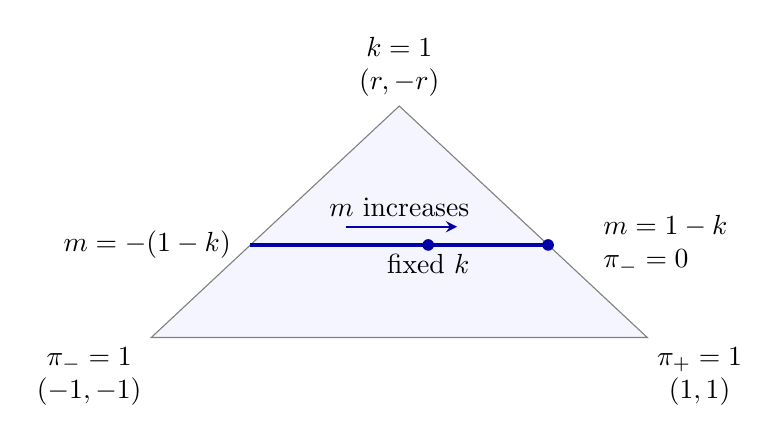
\begin{tikzpicture}[scale=1.05,>=stealth]
\coordinate (N) at (-3,0);
\coordinate (P) at (3,0);
\coordinate (C) at (0,2.8);
\fill[blue!4] (N)--(P)--(C)--cycle;
\draw[gray] (N)--(P)--(C)--cycle;
\node[below left,align=center] at (N) {$\pi_-=1$\\$(-1,-1)$};
\node[below right,align=center] at (P) {$\pi_+=1$\\$(1,1)$};
\node[above,align=center] at (C) {$k=1$\\$(r,-r)$};
\draw[very thick,blue!65!black] (-1.8,1.12)--(1.8,1.12);
\draw[->,thick,blue!65!black] (-.65,1.34)--(.7,1.34);
\node[above] at (0,1.34) {$m$ increases};
\fill[blue!65!black] (.35,1.12) circle (2pt);
\node[below] at (.35,1.12) {fixed $k$};
\fill[blue!65!black] (1.8,1.12) circle (2pt);
\node[right,align=left] at (2.35,1.12) {$m=1-k$\\$\pi_-=0$};
\node[left] at (-1.92,1.12) {$m=-(1-k)$};
\end{tikzpicture}

\caption{Mixture weights for a fixed reflected core $(r,-r)$.
The horizontal segment keeps its mass $k$ fixed, so the separation
$\delta=kr$, entropy $e=kH(r)$, and joining cost $\delta V(r)$ stay fixed.
Moving right increases the mean $m=\pi_+-\pi_-$ until the negative
common output disappears. Theorem~\ref{upgrade:joining} compares the
low-information demand with this endpoint. The triangle is schematic;
its points represent probability weights, not channel values.}
\label{fig:reflected-core}
\end{figure}

Figure~\ref{fig:reflected-core} displays the motion within the reflected
geometry. The path preserves the optimizer's cost and its average
entropy; the original law's individual entropies are retained separately
when applying the local production inequalities.

\section{The deterministic capacity comparison}
\label{capacity:section}

The scalar profile is calibrated at balanced one-bit channels.  At a
biased one-bit channel, the two output labels have unequal posterior
correlations.  Their separation provides the extra reserve needed by
the variance-weighted profile.
The inequality below also follows by differentiating at correlation
one the pointwise one-bit comparison in the proof of
Kramer--Saglam \cite[Lemma~2.4]{KramerSaglam2026}.
We give a direct proof using size-biased posterior information.

\begin{lemma}[A variance-refined one-bit inequality]
\label{capacity:onebit}
Let $g(X)=m+\delta X$, where $X$ is a uniform sign and
$|m|+|\delta|<1$.  Write $\alpha=1-m^2$ and
\[
 J=\frac{\psi(m+\delta)+\psi(m-\delta)}2-\psi(m),
 \qquad D=\frac\delta2\{V(m+\delta)-V(m-\delta)\}.
\]
Then $J<\alpha L$ and
\begin{equation}
 D\ge\alpha F(J/\alpha).
 \label{capacity:refined}
\end{equation}
\end{lemma}

\begin{proof}
Reflection and relabeling allow $m\ge0$, $\delta\ge0$.  The case
$\delta=0$ is immediate, so assume $\delta>0$.  Set
\[
 w_\pm=\frac{1\pm m}{2},\qquad
 r_\pm=\frac\delta{1\pm m},\qquad i_\pm=\psi(r_\pm).
\]
The two posterior representations of the one-bit channel give
\begin{equation}
 J=w_+i_++w_-i_-,\qquad
 D=w_+F(i_+)+w_-F(i_-).
 \label{capacity:posterior}
\end{equation}
For the first identity, introduce a sign $U$ with conditional mean
$g(X)$.  Its probabilities are $w_\pm$, and the conditional means
of $X$ given $U=\pm1$ are $r_+$ and $-r_-$.  Evaluating
$I(U;X)$ in either order gives the identity.  For the second, use
$w_\pm r_\pm=\delta/2$ and
\[
 V(m+\delta)-V(m-\delta)=V(r_+)+V(r_-).
\]

To extract the variance refinement from these identities, use the
secant slope $\varphi(s)=F(s)/s$, with $\varphi(0)=2$.
It is increasing by convexity of $F$ and $F(0)=0$. It is also
convex: the scalar fact $F'''\ge0$ gives, for $s>0$,
\[
 \varphi''(s)
 =\frac{s^2F''(s)-2sF'(s)+2F(s)}{s^3}
 =\frac1{s^3}\int_0^s t^2F'''(t)\,dt\ge0.
\]
Since $\delta>0$, both $i_\pm$ and $J$ are positive.
The size-biased weights $w_\pm i_\pm/J$ therefore sum to one.
Their mean information is
\[
 s_*:=\frac{w_+i_+^2+w_-i_-^2}{J},\qquad
 0<s_*\le\max\{i_+,i_-\}<L.
\]
Jensen's inequality now gives
\begin{equation}
 \frac DJ
 =\frac{w_+i_+}{J}\varphi(i_+)
  +\frac{w_-i_-}{J}\varphi(i_-)
 \ge\varphi(s_*).
 \label{capacity:size-biased}
\end{equation}
It remains to show $s_*\ge J/\alpha$. This will also establish
$J/\alpha<L$ before we evaluate the rate there.

The positive series for $\psi$ shows that $\psi(r)/r^2$ increases.
Consequently
\[
 q:=\frac{i_+}{i_-}
 \le q_0:=\left(\frac{1-m}{1+m}\right)^2.
\]
For $0\le q\le1$, the ratio
\[
 R(q)=\frac{w_+q^2+w_-}{(w_+q+w_-)^2}
\]
decreases, since
\[
 R'(q)=\frac{2w_+w_-(q-1)}{(w_+q+w_-)^3}\le0.
\]
Direct substitution at $q_0$ therefore gives
\begin{equation}
 \frac{w_+i_+^2+w_-i_-^2}{J^2}
 \ge\frac{1+3m^2}{1-m^2}\ge\frac1\alpha.
 \label{capacity:secondmoment}
\end{equation}

Thus $J/\alpha\le s_*<L$. Combining
\eqref{capacity:size-biased} with monotonicity of $\varphi$ yields
\[
 \frac DJ
 \ge\varphi(s_*)
 \ge\varphi(J/\alpha).
\]
This proves both assertions.
\end{proof}


The ordinary one-bit bound follows at once:
\[
 c(m+\delta,m-\delta)\ge\alpha F(J/\alpha)\ge F(J).
\]
The last inequality is convexity with $F(0)=0$ and $0<\alpha\le1$.
We retain the variance-refined form because it pays the deterministic
base of the reserve profile, while its ordinary consequence pays the
information increment at a core.

\section{A reserve that survives adding either common output}
\label{reserve:section}

The linear rate $2I$ leaves a remainder that has a simple behavior
under mixing.  Write $S=F-2I$, as in
\eqref{scalar:surplus-definition}, and put
\begin{equation}
 R(v,e)=vS\!\left(L-\frac ev\right),\qquad v,e>0,
 \label{reserve:perspective}
\end{equation}
using the zero extension of $S$ at negative arguments.  The profile
\eqref{main:profile} is
\[
 \mathcal B_m(I)=2I+R(1-m^2,H(m)-I).
\]
Its construction can be read as an allocation of information between
two capacities.  Set $\alpha=1-m^2$ and
$c_m=H(m)-\alpha L\ge0$.  Then
\begin{equation}
 \mathcal B_m(I)=
 \inf_{\substack{u+v=I\\0\le u\le c_m\\0\le v<\alpha L}}
 \{2u+\alpha F(v/\alpha)\},\qquad 0\le I<H(m).
 \label{reserve:allocation}
\end{equation}
Indeed, $F'\ge2$ makes the optimum $u=\min\{I,c_m\}$.
The capacity $c_m$ is paid at the linear rate, while the remaining
capacity $\alpha L$ uses the exact coordinate rate.  This is an
identity for the profile, not a decomposition of an actual channel.
The finite-noise bound of Kramer and Saglam
\cite[Theorem~1.1]{KramerSaglam2026} reads, in the present
normalization,
\[
 I(T_\rho f)\le\rho^2c_m+\alpha\psi(\rho)
 \qquad(0\le\rho\le1)
\]
for a Boolean field $f$ on the uniform cube with $\E f=m$.
It uses the same coefficients $\alpha$ and $c_m$; here they
define the local production profile $\mathcal B_m$.

To determine the payment required by a join, consider a physical state
\[
 |m|+\delta<1,\quad\delta\ge0,\quad
 0<e\le\bar h:=\frac{H(m+\delta)+H(m-\delta)}2,
\]
and write
\[
 \alpha=1-m^2,\quad\beta=\alpha-\delta^2,
 \qquad J=H(m)-\bar h,\quad j=\bar h-e.
\]
Set $a=m+\delta$ and $b=m-\delta$.  Let $e_a,e_b>0$ satisfy
$e_a\le H(a)$, $e_b\le H(b)$, and $(e_a+e_b)/2=e$, and put
$I_a=H(a)-e_a$, $I_b=H(b)-e_b$.  Their average information is
$j$, and their average variance capacity is
$[(1-a^2)+(1-b^2)]/2=\beta$.  Since $R$ is a convex
perspective, the child profiles satisfy
\begin{equation}
 \frac{\mathcal B_a(I_a)+\mathcal B_b(I_b)}2
 \ge2j+R(\beta,e).
 \label{reserve:pooling}
\end{equation}
The parent information is $I=H(m)-e=J+j$.  Subtracting the
pooled bound from $\mathcal B_m(I)=2(J+j)+R(\alpha,e)$ gives
the required payment
\begin{equation}
 W(m,\delta,e)=2J+R(\alpha,e)-R(\beta,e).
 \label{reserve:payment}
\end{equation}
Thus
\[
 \mathcal B_m(I)-\frac{\mathcal B_a(I_a)+\mathcal B_b(I_b)}2
 \le W(m,\delta,e).
\]
It is enough to prove $W\le\mathcal K$.  The deterministic
capacity comparison pays the interior core; the next two lemmas
show that this payment survives adding either common output.

\subsection{A logarithmic bound for the corner geometry}

\begin{lemma}
\label{reserve:geometry}
For $-1<m<1$ and $0\le\delta<1-|m|$, put
\[
 A=1-m,\qquad
 \kappa=\frac12\log\frac1{1-\delta^2/(1+m)^2}.
\]
Then
\begin{equation}
 A^2\log\frac\alpha\beta\le3\kappa.
 \label{reserve:log-geometry}
\end{equation}
\end{lemma}

\begin{proof}
The case $\delta=0$ is immediate.  Otherwise set
\[
 h=\frac{1-m}{1+m}>0,\qquad
 t=\frac{\delta^2}{(1+m)^2}<\min\{1,h^2\},\qquad
 f(t)=-\log(1-t).
\]
The ratio $f(t/h)/f(t)$ decreases in $t$ when $h\ge1$ and
increases when $h\le1$.  Indeed, the ratio of the corresponding
positive integrands is $(1-t)/(h-t)$, whose derivative has sign
$1-h$; the same monotonicity passes to their integral ratio.

If $h\ge1$, the ratio is at most its limit $1/h$ at zero.
Thus $A^2f(t/h)/f(t)\le A^2/h=1-m^2\le1$.
If $0<h<1$, it suffices to bound the ratio at $t=h^2$.
The function
\[
 G(h)=(2-h)f(h)-(2+h)\log(1+h)
\]
has $G(0)=0$ and
\[
 G'(h)=2\left[\frac h{1-h^2}-V(h)\right]>0.
\]
The last sign follows by bounding the integral defining $V(h)$
by its endpoint integrand.  Consequently
\[
 \frac{f(h^2)}{f(h)}
 =1-\frac{\log(1+h)}{f(h)}\ge\frac{2h}{2+h},
\]
and
\[
 A^2\frac{f(h)}{f(h^2)}
 \le\frac{2h(2+h)}{(1+h)^2}
 =2-\frac2{(1+h)^2}\le\frac32.
\]
Since $f(t)=2\kappa$ and $f(t/h)=\log(\alpha/\beta)$,
both cases give \eqref{reserve:log-geometry}.
\end{proof}

\subsection{The common-output contraction}

\begin{lemma}[Adding either common output]
\label{reserve:corner}
For every physical state $(m,\delta,e)$ and $0<\tau\le1$,
\begin{equation}
 W(1-\tau+\tau m,\tau\delta,\tau e)
 \le\tau W(m,\delta,e).
 \label{reserve:plus-corner}
\end{equation}
The same inequality holds with parent mean $-1+\tau+\tau m$,
corresponding to the negative common output.  There is no sign
restriction on the original mean.
\end{lemma}

\begin{proof}
The positive-corner ray scales $A=1-m$, $\delta$, and $e$ by
the same factor.  Hold $\delta/A$ and $e/A$ fixed, and put
$\eta=1+\delta^2/A^2$.  Entropy differentiation gives
\begin{equation}
 A\frac{dJ}{dA}-J=\kappa.
 \label{reserve:entropy-euler}
\end{equation}
To check this identity, use
$H(m)-(1-m)V(m)=\log[2/(1+m)]$; the average of the two
child logarithms is the parent logarithm plus $\kappa$.

For $h>0$, define the entropy intercept
\[
 \gamma(h)=S(L-h)+hS'(L-h)
 =\begin{cases}
 \displaystyle\int_h^L\frac{P(u)}u\,du,&0<h<L,\\
 0,&h\ge L,
 \end{cases}
 \qquad P(u)=u^2F''(L-u).
\]
By the scalar curvature bound, $P\le M=4L^2/3$ and $2>3M$.
Thus $\gamma\ge0$, and
\begin{equation}
 0\le\gamma(e/\alpha)-\gamma(e/\beta)
 \le M\log\frac\alpha\beta.
 \label{reserve:intercept-bound}
\end{equation}
If an argument crosses the clipping point, the integral is simply
truncated at $L$.

Since $\alpha=A(2-A)$ and $\beta=A(2-\eta A)$, differentiation
of the perspectives in \eqref{reserve:payment} gives
\begin{equation}
 A\frac{dW}{dA}-W
 =2\kappa+A^2\{\eta\gamma(e/\beta)-\gamma(e/\alpha)\}.
 \label{reserve:euler}
\end{equation}
For example, with $e=Az$, one has
$R(\alpha,e)/A=(2-A)S(L-z/(2-A))$, whose derivative is
$-\gamma(e/\alpha)$.  The second perspective gives the factor
$\eta$.  The clipped remainder is $C^1$, because $S(0)=S'(0)=0$,
so these identities hold across the seam; no second derivative of
the zero extension is needed.

Now $\eta\ge1$, \eqref{reserve:intercept-bound}, and
Lemma~\ref{reserve:geometry} give the whole comparison:
\begin{equation}
 A\frac{dW}{dA}-W
 \ge2\kappa-MA^2\log\frac\alpha\beta
 \ge(2-3M)\kappa\ge0.
 \label{reserve:corner-margin}
\end{equation}
Therefore $W/A$ is nondecreasing.  Comparing $A$ and $\tau A$
proves \eqref{reserve:plus-corner}.  The intermediate states remain
physical by entropy concavity, and all child means stay interior for
$\tau>0$.  Finally $W$ is even in $m$, so reflection proves the
negative-corner statement.  For $\delta=0$, every displayed payment
and margin is zero.
\end{proof}

\subsection{From one core to the local inequality}

\begin{theorem}[Local joining for the linear reserve]
\label{reserve:joining}
Let $(A,B)$ have any joint law on $[-1,1]^2$ with
$e_a=\E H(A)>0$ and $e_b=\E H(B)>0$.  Put
\[
 a=\E A,\quad b=\E B,\quad m=\frac{a+b}{2},
 \quad e=\frac{e_a+e_b}{2},
\]
and $I=H(m)-e$, $I_a=H(a)-e_a$, $I_b=H(b)-e_b$.  Then
\begin{equation}
 \E c(A,B)\ge
 \mathcal B_m(I)-\frac{\mathcal B_a(I_a)+\mathcal B_b(I_b)}2.
 \label{reserve:local-bound}
\end{equation}
\end{theorem}

\begin{proof}
An infinite cost is immediate.  Otherwise positive child entropies
give interior means.  Swap the children if necessary so that
$\delta=(a-b)/2\ge0$; entropy concavity makes $(m,\delta,e)$
physical.

First pay the deterministic capacity state.  For an interior pair
$x,y$, let $m_0=(x+y)/2$, $\delta_0=|x-y|/2$,
$e_0=[H(x)+H(y)]/2$, and $J_0=H(m_0)-e_0$.
Write $\alpha_0=1-m_0^2$, $\beta_0=\alpha_0-\delta_0^2$.
The entropy lower bound gives $e_0\ge\beta_0L$ and
\[
 [L-e_0/\alpha_0]_+\le J_0/\alpha_0<L.
\]
The last strict inequality and the variance-refined one-bit bound
are Lemma~\ref{capacity:onebit}.  Hence
\begin{equation}
 \begin{aligned}
 W(m_0,\delta_0,e_0)
 &=2J_0+\alpha_0S(L-e_0/\alpha_0)\\
 &\le2J_0+\alpha_0S(J_0/\alpha_0)
 =\alpha_0F(J_0/\alpha_0)\le c(x,y).
 \end{aligned}
 \label{reserve:capacity}
\end{equation}

For $\delta>0$, Proposition~\ref{canonical:coverage} supplies
an exact optimizer with interior core $(x,y)$ of mass $k>0$
and equal-corner masses $\pi_+,\pi_-$, where
$k+\pi_++\pi_-=1$.  Its cost is $k c(x,y)$.
Starting from the core, add the positive corner with retention
factor $k/(k+\pi_+)$, then the negative corner with retention
factor $k+\pi_+$.  These two operations produce exactly the
canonical law.  Lemma~\ref{reserve:corner} and
\eqref{reserve:capacity} give
\begin{equation}
 W(m,\delta,e)
 \le(k+\pi_+)\frac{k}{k+\pi_+}W(m_0,\delta_0,e_0)
 \le k c(x,y)=\mathcal K(m,\delta,e).
 \label{reserve:canonical-payment}
\end{equation}
Both retention factors are positive; a missing corner gives a
factor one.  No orientation or separate case for the core is required.
For $\delta=0$, $W=\mathcal K=0$ directly.

Finally the actual pair law has cost at least
$\mathcal K(m,\delta,e)$.  Combining
\eqref{reserve:canonical-payment} with the original-child pooling
bound \eqref{reserve:pooling} gives
\[
 \E c(A,B)+\frac{\mathcal B_a(I_a)+\mathcal B_b(I_b)}2
 \ge2(J+j)+R(\alpha,e)=\mathcal B_m(I).
\]
All child profiles use their original individual entropies; only
the joining cost was minimized with their common average budget.
\end{proof}

The pooling step has a useful exact interpretation.  If
$e<\beta L$, its minimum over the entropy split is attained at
$e_a/(1-a^2)=e_b/(1-b^2)=e/\beta$; these entropies are
physical because $H(a)\ge(1-a^2)L$, and similarly for $b$.
If $e\ge\beta L$, allocate both child entropies in the intervals
$[(1-a^2)L,H(a)]$ and $[(1-b^2)L,H(b)]$ with the prescribed
average.  Both remainders vanish.  Thus the perspective in
\eqref{reserve:pooling} is the exact common-budget value of the
child reserve, rather than an additional approximation.

\section{Paying the information increment by thinning}
\label{thinning:section}

The canonical optimizer with one positive common corner has a useful
feature: its cost is linear in the mass of its interior core.  We will
show that the information-rate increment is at most the core's
increment multiplied by that mass.  At full mass the increment is
paid by the one-bit posterior comparison.  This will settle the whole
high-entropy branch of the canonical cost problem.

The scalar inputs already proved here are
\begin{equation}
\label{thinning:scalar-inputs}
 F(0)=0,\qquad F'(I)\ge2,\qquad
 0<F''(I)\le\frac{M}{(L-I)^2},\qquad
 M=\frac{4L^2}{3},\qquad 2>3M.
\end{equation}
Indeed, the slope follows from
Lemma~\ref{scalar:profile-convexity}, the curvature bound from
Lemma~\ref{scalar:scaled-curvature}, and the strict margin from
Lemma~\ref{scalar:entropy-bounds}.  The proof isolates the roles of
these two bounds: the slope supplies a positive term, while the
curvature controls the possible loss over an entropy interval.

\subsection{The common-output path}

Fix an interior ordered pair $a_c>b_c$ with nonnegative center, and
write
\[
 x_c=\frac{a_c+b_c}{2}\ge0,\qquad
 d_c=\frac{a_c-b_c}{2}>0,\qquad
 h_c=\frac{H(a_c)+H(b_c)}2,\qquad
 J_c=H(x_c)-h_c.
\]
For $0<\lambda\le1$, put mass $\lambda$ on this core and mass
$1-\lambda$ on $(1,1)$.  The second atom is a common output: its
coordinates agree, and it contributes neither entropy nor cost.  The
mixture has means $x+d$ and $x-d$, where
\begin{equation}
\label{thinning:path}
 x=1-\lambda(1-x_c),\qquad d=\lambda d_c,
 \qquad e=\lambda h_c.
\end{equation}
For this path define
\begin{equation}
\label{thinning:information}
 \bar h=\frac{H(x+d)+H(x-d)}2,\qquad
 \nu=\bar h-e,\qquad J=H(x)-\bar h,
 \qquad I=\nu+J=H(x)-e.
\end{equation}
The average child information is $\nu$, and $J$ is the entropy gained
by averaging the two child means.  Since
$0<d_c<1-x_c\le1$, the mixture has $x\ge0$ and
$0<d<1-x$.  Entropy concavity gives $\nu\ge0$; strict concavity
gives $J>0$; and $e>0$ gives $I<L$.  Thus every rate argument lies
in $[0,L)$.

These quantities have a channel interpretation.  Let $X$ be a fair
sign and let $B\in\{0,1\}$ be an independent flag with
$\Pr(B=1)=\lambda$.  Given $X,B$, draw a sign $U$ with conditional mean
\[
 \E[U\mid X,B]=(1-B)+B(x_c+d_cX).
\]
Thus $B=0$ selects the common output and $B=1$ selects the core.
The three relevant entropies are
$H(U)=H(x)$, $H(U\mid X)=\bar h$, and
$H(U\mid X,B)=e$.  The chain rule therefore reads
\begin{equation}
\label{thinning:flag-information}
 I=I(U;X,B),\qquad \nu=I(U;B\mid X),\qquad
 J=I(U;X),\qquad I=\nu+J.
\end{equation}
In particular, $\nu$ is the information about the flag after the
input has been revealed.

\begin{theorem}[Common-output payment]
\label{thinning:payment}
For the core and mass in \eqref{thinning:path},
\begin{equation}
\label{thinning:value}
 F(\nu+J)-F(\nu)\le\lambda F(J_c).
\end{equation}
\end{theorem}

We prove this by showing that $[F(\nu+J)-F(\nu)]/\lambda$
increases with $\lambda$. This normalization matches the mixture's
cost $\lambda c(a_c,b_c)$. We first compute its derivative and
identify the entropy-interval estimate that makes it nonnegative.

\subsection{The normalized derivative}

For the state \eqref{thinning:path}, set
\begin{equation}
\label{thinning:window-data}
 \begin{gathered}
 p=1+x,\qquad \sigma=1-x,\qquad b=\log(1+x),\\
 q=e+\psi(x)=L-I,\qquad s=e+L-\bar h=L-\nu,\\
 \kappa=-\frac12\log\left(1-\frac{d^2}{p^2}\right)>0.
 \end{gathered}
\end{equation}
In particular $s-q=J$ and $0<q<s\le L$. Write
\[
 \Delta(\lambda)=F(I)-F(\nu),\qquad
 A=\log\frac2{1+x}=L-b.
\]
For $h_{\mathrm{bin}}(t)=H(1-2t)$, the entropy identity is
\[
 t h_{\mathrm{bin}}'(t)-h_{\mathrm{bin}}(t)=\log(1-t).
\]
Apply it first to
$I=h_{\mathrm{bin}}(\lambda(1-x_c)/2)-\lambda h_c$,
then to the two child expressions with initial probabilities
$(1-a_c)/2$ and $(1-b_c)/2$, and average. The result is
\begin{equation}
\label{thinning:path-derivatives}
 \lambda I'=I-A,\qquad
 \lambda\nu'=\nu-A-\kappa.
\end{equation}
For the second identity, the two logarithms have average
\[
 \frac12\log\frac{(1+x)^2-d^2}{4}=-A-\kappa.
\]

Substitution gives the exact Euler derivative
\begin{equation}
\label{thinning:normalized-derivative}
 \lambda\Delta'-\Delta
 =\int_\nu^I(u-A)F''(u)\,du+F'(\nu)\kappa.
\end{equation}
Indeed, at the chosen value of $\lambda$, the derivative in $u$
of $(u-A)F'(u)-F(u)$ is $(u-A)F''(u)$. The value of $A$ is
held fixed only during this auxiliary integration; both path
derivatives have already been included.

The last term in \eqref{thinning:normalized-derivative} is at least
$2\kappa$. Convexity makes the integrand nonnegative where $u\ge A$.
On the remaining part, the curvature bound
$F''(u)\le M/(L-u)^2$ and the substitution $h=L-u$ give
\begin{equation}
\label{thinning:derivative-loss}
 \lambda\Delta'-\Delta
 \ge2\kappa-M\int_q^s\frac{(h-b)_+}{h^2}\,dh.
\end{equation}
Thus it suffices to prove that this integral is at most $3\kappa$:
the strict margin $2>3M$ will then make
$(\Delta/\lambda)'$ nonnegative. The cutoff $b$ marks exactly
the part of the entropy interval where the curvature term can be
negative. We will first prove an interval estimate for this kernel,
then check its hypotheses using the entropy of the core.

The positive term also has a channel interpretation. For the channel
in \eqref{thinning:flag-information}, the posterior of the fair input
at the positive output is
\[
 \Pr(X=z\mid U=1)=\frac12\left(1+\frac{zd}{p}\right),
 \qquad z\in\{-1,1\}.
\]
Consequently
\[
 \kappa=\frac12\sum_{z=\pm1}
 \log\frac{1/2}{\Pr(X=z\mid U=1)}
 =D_{\mathrm{KL}}\!\left(
 \operatorname{Unif}\{-1,1\}\,\middle\|\,
 \mathcal L(X\mid U=1)\right).
\]
This is the relative entropy from the prior to the positive-output
posterior, with the flag marginalized. It is an auxiliary path
quantity, distinct from the canonical cost $\mathcal K$.

\subsection{An estimate for entropy intervals}

\begin{lemma}[An interval estimate with a logarithmic cutoff]
\label{thinning:interval}
Let $0\le x<1$, and put
\[
 p=1+x,\qquad \sigma=1-x,\qquad
 \gamma=\frac{\sigma}{p},\qquad
 \beta=\frac{\log(1+x)}L.
\]
Suppose
\[
 0\le z<\gamma,\qquad \sigma-pz\le u\le1-z.
\]
For $\beta>0$, define $k_\beta(v)=(v-\beta)_+/v^2$ for $v>0$
and $k_\beta(0)=0$.  For $\beta=0$, set $k_0(v)=1/v$ for $v>0$.
Then
\begin{equation}
\label{thinning:interval-bound}
 \int_u^{u+z}k_\beta(v)\,dv
 \le-\frac32\log(1-\gamma z).
\end{equation}
If $x>0$, the endpoint $z=\gamma$ is also allowed.  At $z=0$,
both sides are zero.
\end{lemma}

\begin{proof}
We first bound the cutoff by a rational function:
\begin{equation}
\label{thinning:cutoff-bound}
 \beta\ge b_*:=\frac{4x}{3+x},\qquad
 1-\beta\le\frac{3\sigma}{3+x}\le\frac32\gamma.
\end{equation}
For $0<x\le1$, let $R(x)=(3+x)\log(1+x)/x$.  Direct
differentiation gives
\[
 x^2R'(x)=N(x):=\frac{x(3+x)}{1+x}-3\log(1+x),
 \qquad N'(x)=-\frac{x(1-x)}{(1+x)^2}\le0.
\]
Since $N(0)=0$, $R$ decreases and $R(x)\ge R(1)=4L$.
This proves the first inequality, including $x=0$ by continuity.
The other two follow from $1-b_*=3\sigma/(3+x)$ and $x\le1$.

Consider an admissible interval $[u,u+z]$ with $z<\gamma$.
The constraints imply
\[
 a:=\frac{2-u}{1+z}\in[1,p].
\]
Keep this $a$ and the cutoff $\beta$ fixed, and consider the affine
family of intervals
\begin{equation}
\label{thinning:affine-intervals}
 u_a(s)=2-a(1+s),\qquad v_a(s)=u_a(s)+s,
 \qquad 0\le s\le z.
\end{equation}
Because $1\le a\le p$, these intervals satisfy
\[
 0<\sigma-ps\le u_a(s)\le v_a(s)\le1.
\]
The initial interval has length zero; the final one is $[u,u+z]$.
The Leibniz rule gives
\[
 \frac{d}{ds}\int_{u_a(s)}^{v_a(s)}k_\beta(v)\,dv
 =D_a(s):=a k_\beta(u_a(s))-(a-1)k_\beta(v_a(s)).
\]
We claim that
\begin{equation}
\label{thinning:interval-derivative}
 D_a(s)\le\frac{3\gamma}{2(1-\gamma s)}.
\end{equation}

For this estimate, abbreviate $u=u_a(s)$ and $v=v_a(s)$.
Above the cutoff,
$k_\beta'(v)=(2\beta-v)/v^3$; thus $k_\beta$ first increases
and then decreases, with the decreasing case $\beta=0$ included.
Its minimum on $[u,1]$ is at an endpoint.  Consequently
\[
 k_\beta(v)\ge\min\{k_\beta(u),1-\beta\}.
\]
If $k_\beta(u)\le1-\beta$, this gives
$D_a\le k_\beta(u)\le1-\beta$, and
\eqref{thinning:interval-derivative} follows from
\eqref{thinning:cutoff-bound}.

Otherwise set $A_*=k_\beta(u)-(1-\beta)>0$.  Then $u>\beta$,
and
\[
 D_a\le aA_*+(1-\beta),\qquad
 Y:=\frac{1-\gamma s}{\gamma}
 =\frac2\sigma-\frac{2-u}{a}>0.
\]
To bound their product, hold $u,\beta,x$ fixed and vary $a$ in
the algebraic expression
\[
 \Theta(a)=\{aA_*+(1-\beta)\}
 \left\{\frac2\sigma-\frac{2-u}{a}\right\}.
\]
It increases with $a$, since
\[
 \Theta'(a)=\frac{2A_*}{\sigma}
 +\frac{(2-u)(1-\beta)}{a^2}>0.
\]
The actual value has $a\le p$, so
\begin{equation}
\label{thinning:transport-bound}
 YD_a\le\Theta(p)
 =\{p k_\beta(u)-x(1-\beta)\}
   \frac{4x+\sigma u}{\sigma p}.
\end{equation}
This last expression decreases with $\beta$: its positive factor
is independent of $\beta$, and the first factor has derivative
$-p/u^2+x<0$.  Since $u>\beta\ge b_*$, replacing $\beta$ by
$b_*$ keeps $u$ above the cutoff and gives an upper bound.
The hard-case condition also gives
\[
 u^2\{k_\beta(u)-(1-\beta)\}
 =(1-u)\{(1-\beta)u-\beta\}>0.
\]
Thus $u<1$ and
$u>\beta/(1-\beta)\ge b_*/(1-b_*)$.
Putting $t=b_*/u$ now yields $0\le t<1/(1+u)$.
Using $x=3b_*/(4-b_*)$, substitution and a common denominator give
\[
 \frac32-\left.\Theta(p)\right|_{\beta=b_*}
 =\frac{\mathcal P(t,u)}{2(1-tu)(2+tu)},
\]
where the numerator satisfies
\begin{equation}
\label{thinning:polynomial}
 \begin{split}
 \mathcal P(t,u):={}&3(2-tu-t^2u^2)\\
 &-\{2(2+tu)(1-t)-3tu^2(1-tu)\}\{1+t(3-u)\}\ge0,
 \qquad 0\le u\le1,\quad 0\le t\le\frac1{1+u}.
 \end{split}
\end{equation}
To prove this polynomial inequality, put
\[
 C_2=12-8u+8u^2-6u^3,\qquad C_1=3u^2-u-8,\qquad
 C_3=u(3-u)(2-3u^2).
\]
Expansion gives
\begin{equation}
\label{thinning:polynomial-decomposition}
 \mathcal P=2+C_1t+C_2t^2+C_3t^3.
\end{equation}
Since
\[
 C_3+u(1+u)=u(1-u)(7+6u-3u^2)\ge0,
 \qquad t(1+u)\le1,
\]
we have $C_3t\ge-u$: this is immediate for $C_3\ge0$, while for
$C_3<0$ it follows from $C_3\ge-u(1+u)$ and $t\le1/(1+u)$.
Hence $\mathcal P\ge2+C_1t+(C_2-u)t^2$.
The exact identity
\[
 8(C_2-u)-C_1^2
 =4+(1-u)\{2(5u-3)^2+u^2(1+9u)+10\}\ge4
\]
therefore gives
\[
 8\mathcal P\ge(4+C_1t)^2+4t^2>0.
\]
This proves \eqref{thinning:polynomial}, including $t=0$.
The denominator in the preceding gap is positive because
$tu=b_*<1$. Thus $YD_a\le3/2$,
which is \eqref{thinning:interval-derivative}.
Integrating from $0$ to $z$ proves \eqref{thinning:interval-bound}.

For $x=0$, admissibility forces $a=1$ and the family is
$[1-s,1]$, whose lower endpoint is positive for $s<1$.  The
integrand $k_0(v)=1/v$ therefore causes no endpoint problem.
For $x>0$, the cutoff is positive and $k_\beta$ is continuous at
zero with the stated extension.  Also $\gamma<1$, so continuity
along the same family extends the bound to $z=\gamma$.
The zero-length case is immediate.
\end{proof}

\subsection{The entropy interval of the channel}

We now return to the quantities in \eqref{thinning:window-data}.
To apply the interval estimate to $[q,s]$, we need a lower bound
on its position and an upper bound on its length $J$. Both follow
from the entropy of the oriented core.

\begin{lemma}[The entropy interval on a thinning path]
\label{thinning:window}
Every state on \eqref{thinning:path} satisfies
\begin{equation}
\label{thinning:window-bound}
 \int_q^s\frac{(h-b)_+}{h^2}\,dh\le3\kappa.
\end{equation}
\end{lemma}

\begin{proof}
The nonnegative center of the core supplies the essential lower
entropy bound.  Write $h_{\mathrm{bin}}(t)=H(1-2t)$, let
$\sigma_c=1-x_c\le1$, and put
\[
 t=\frac{1-d_c/\sigma_c}{2}\in(0,1/2).
\]
The two negative-output probabilities at the core are
$\sigma_c t$ and $\sigma_c(1-t)$.  Concavity and
$h_{\mathrm{bin}}(0)=0$ imply
\[
 h_{\mathrm{bin}}(\sigma_c t)\ge\sigma_c h_{\mathrm{bin}}(t),\qquad
 h_{\mathrm{bin}}(\sigma_c(1-t))
 \ge\sigma_c h_{\mathrm{bin}}(1-t)=\sigma_c h_{\mathrm{bin}}(t).
\]
Averaging and multiplying by $\lambda$, with
$\sigma=\lambda\sigma_c$ and $d/\sigma=d_c/\sigma_c$, gives
\begin{equation}
\label{thinning:entropy-floor}
 e\ge\sigma H(d/\sigma).
\end{equation}
This is a consequence of the oriented common-output path; it is not
an assertion about every pair law with the same means.
The bound $H(r)\ge L(1-r^2)$ in
Lemma~\ref{scalar:entropy-bounds} now yields
\begin{equation}
\label{thinning:quadratic-floor}
 q\ge e\ge L\left(\sigma-\frac{d^2}{\sigma}\right).
\end{equation}

Expanding the binary entropies in $J$ gives the posterior identity
\[
 J=\frac p2\psi(d/p)+\frac\sigma2\psi(d/\sigma).
\]
Using $\psi(r)\le Lr^2$ on both terms, we obtain
\[
 J\le\frac{Ld^2}{\sigma p}=:Lz,\qquad
 0<z<\frac\sigma p.
\]
The upper bound on $z$ follows from $d<\sigma$.  Together with
\eqref{thinning:quadratic-floor}, these estimates say
\[
 q\ge L(\sigma-pz),\qquad q+J=s\le L,
 \qquad L(\sigma-pz)+Lz=L(\sigma-xz)\le L.
\]
We may therefore enlarge $[q,s]$ to an interval of length $Lz$
inside $[L(\sigma-pz),L]$.  More explicitly, choose its lower
endpoint as $q_*:=\min\{q,L-Lz\}$.  Both candidates are at least
$L(\sigma-pz)$, and $q_*\le q$; its upper endpoint is either
$q+Lz\ge s$ or $L\ge s$.  The integrand is nonnegative, so this
enlargement can only increase the integral.

Rescale $h=Lv$.  With $\beta=b/L$ the integrand becomes
$k_\beta(v)\,dv$, with no additional factor of $L$.  The lower
endpoint $q_*/L$ and length $z$ satisfy
Lemma~\ref{thinning:interval} for this $x$ and
$\gamma=\sigma/p$.  Hence
\[
 \int_q^s\frac{(h-b)_+}{h^2}\,dh
 \le-\frac32\log(1-\gamma z)
 =-\frac32\log\left(1-\frac{d^2}{p^2}\right)
 =3\kappa.
\]
This includes $x=0$, which on the path can occur only at
$\lambda=1$, $x_c=0$.
\end{proof}

\begin{proof}[Proof of Theorem~\ref{thinning:payment}]
Combine the derivative reduction \eqref{thinning:derivative-loss}
with Lemma~\ref{thinning:window}:
\begin{align*}
 \lambda\Delta'-\Delta
 &\ge2\kappa-M\int_q^s\frac{(h-b)_+}{h^2}\,dh\\
 &\ge(2-3M)\kappa\ge0.
\end{align*}
Thus
$(\Delta/\lambda)'=(\lambda\Delta'-\Delta)/\lambda^2\ge0$.
At $\lambda=1$, the flag is deterministic, so $\nu=0$, $I=J_c$,
and $\Delta=F(J_c)$.  Comparing with this endpoint proves
\eqref{thinning:value}.  No limit as $\lambda$ tends to zero is needed.
\end{proof}

\subsection{The canonical high-entropy value}

\begin{theorem}[The canonical high-entropy value comparison]
\label{thinning:high-value}
Let $x\ge0$, $d>0$, and $x+d<1$.  Define
\[
 \bar h(x,d)=\frac{H(x+d)+H(x-d)}2,\qquad
 e_0(x,d)=(1-x)H\!\left(\frac d{1-x}\right).
\]
For every $e_0(x,d)\le e\le\bar h(x,d)$,
\begin{equation}
\label{thinning:high-value-bound}
 \mathcal K(x,d,e)\ge
 J_0(x,d,e):=F(H(x)-e)-F(\bar h(x,d)-e).
\end{equation}
\end{theorem}

\begin{proof}
The canonical classification at \eqref{canonical:transition} represents
every state in this closed high-entropy branch by
\eqref{thinning:path}, with a nonnegative core center and
$\mathcal K(x,d,e)=\lambda c(a_c,b_c)$.
Put $\alpha_c=1-x_c^2$.  Lemma~\ref{capacity:onebit} and convexity
of $F$, with $F(0)=0$, give
\[
 c(a_c,b_c)\ge\alpha_c F(J_c/\alpha_c)\ge F(J_c).
\]
Theorem~\ref{thinning:payment} therefore implies
\[
 J_0(x,d,e)=F(\nu+J)-F(\nu)
 \le\lambda F(J_c)
 \le\lambda c(a_c,b_c)=\mathcal K(x,d,e).
\]
\end{proof}

The canonical optimizer is used here only to evaluate a lower bound
on joining cost.  For an original pair law with means $x\pm d$ and
individual entropies $e_a,e_b$, the value of $e$ in
\eqref{thinning:high-value-bound} is their actual average.  The
original child information values remain $H(x+d)-e_a$ and
$H(x-d)-e_b$; their average is $\bar h(x,d)-e$.
Convexity of $F$ therefore gives the common floor at those original
child states:
\[
 \frac{F(H(x+d)-e_a)+F(H(x-d)-e_b)}2
 \ge F(\bar h(x,d)-e).
\]
No individual entropy moment of the canonical law is substituted for
either original child entropy.

\section{From the linear reserve to the sharp rate}
\label{upgrade:section}

The local reserve inequality does not by itself give the sharp rate
$F(I)$ at every state. We now join their maximum
\[
 \widehat{\mathcal B}_m(I)
 =\max\{\mathcal B_m(I),F(I)\}.
\]
Closure under a maximum is a useful feature of the local-production
framework \cite[Lemma~3]{ChenGohariNair2025}, but $F$ alone does not
satisfy a joining inequality for every law. We therefore prove the
needed comparison in the part of the domain where the reserve is
insufficient. Two comparisons organize the proof. Above half information, the
reserve already dominates $F$. Below half information, the demand
from $F$ increases with the common mean of the child states. Thus
every reflected core can be paid at its one-corner wall by the same
thinning theorem used for a one-corner optimizer.

\subsection{The reserve above half information}

\begin{lemma}[The high-information reserve]
\label{upgrade:high-information}
For $|m|<1$ and $L/2\le I<H(m)$,
\begin{equation}
 \mathcal B_m(I)\ge F(I).
 \label{upgrade:high-information-bound}
\end{equation}
The inequality is strict if $m\ne0$. Consequently a state with
$F(I)>\mathcal B_m(I)$ must have $I<L/2$.
\end{lemma}

\begin{proof}
Recall $S(I)=F(I)-2I$ on $[0,L)$ and put
\[
 k_0=L-\frac12,\qquad
 \Xi(I)=(I-k_0)S'(I)-S(I).
\]
Since $S(0)=S'(0)=0$ and $S''=F''$ on this interval,
\begin{equation}
 \Xi(I)=\int_0^I(s-k_0)F''(s)\,ds.
 \label{upgrade:centered-curvature}
\end{equation}
Lemma~\ref{scalar:curvature-growth} says that
$w(s)=e^{-2s}F''(s)$ strictly increases. Also
$0<k_0<L/2$, and the binary identity $e^L=2$ gives the exact
balance
\begin{equation}
 \int_0^{L/2}(s-k_0)e^{2s}\,ds
 =\left[\frac12e^{2s}(s-L)\right]_0^{L/2}=0.
 \label{upgrade:exponential-balance}
\end{equation}
On the part of the integral below $k_0$, the factor $s-k_0$ is
negative and $w(s)\le w(k_0)$. Above $k_0$, one has
$s-k_0>0$ and $w(s)\ge w(k_0)$. Replacing $w(s)$ by $w(k_0)$
therefore gives a lower
bound on both parts, strictly so on intervals of positive length.
Equations \eqref{upgrade:centered-curvature}--
\eqref{upgrade:exponential-balance} imply
\[
 \Xi(L/2)
 =\int_0^{L/2}(s-k_0)e^{2s}w(s)\,ds>0.
\]
Since $\Xi'(I)=(I-k_0)F''(I)>0$ for $I\ge L/2$, we have
$\Xi(I)>0$ throughout that range.

For the mean-dependent comparison, set
\[
 \alpha=1-m^2,\qquad
 c_m=H(m)-\alpha L=Lm^2-\psi(m).
\]
The elementary entropy bounds give
$0\le c_m\le m^2k_0$. Hence, for $I\ge L/2$, the argument
\[
 s=L-\frac{H(m)-I}{\alpha}
   =\frac{I-c_m}{\alpha}
\]
is positive; it is less than $L$ because $I<H(m)$. No clipping
occurs in this comparison. The tangent inequality for the convex
function $S$, and $S'\ge0$, now yield
\begin{align*}
 \mathcal B_m(I)-F(I)
 &=\alpha S(s)-S(I)\\
 &\ge\alpha[S(I)+(s-I)S'(I)]-S(I)\\
 &=m^2[IS'(I)-S(I)]-c_mS'(I)\\
 &\ge m^2[(I-k_0)S'(I)-S(I)]
 =m^2\Xi(I)\ge0.
\end{align*}
The inequality is strict at a nonzero mean. At mean zero,
$\alpha=1$, $c_m=0$, and the two profiles agree identically.
\end{proof}

\subsection{A direct comparison with the one-corner wall}

\begin{lemma}[The demand below half information]
\label{wall:monotonicity}
Let $m,d>0$, $m+d<1$, and
\[
 0<e\le\bar h(m,d):=\frac{H(m+d)+H(m-d)}2.
\]
Put $I=H(m)-e$, $j=\bar h(m,d)-e$, and $J=I-j$. If
$I\le L/2$, then at fixed $d,e$,
\begin{equation}
 \partial_m\{F(I)-F(j)\}>0.
 \label{wall:positive-derivative}
\end{equation}
At $j=0$, the derivative is interpreted from the physical side.
\end{lemma}

\begin{proof}
We compare the rate slopes with the entropy slopes. First,
\begin{equation}
 \frac{F''(u)}{F'(u)}<2\qquad(0\le u\le L/2).
 \label{wall:rate-slope}
\end{equation}
Indeed, set $h=L-u\ge L/2$. The lower bound
$F''(u)\ge1/[2(L-u)^2]$ from
Lemma~\ref{scalar:scaled-curvature} gives
\[
 F'(u)\ge2+\frac12\left(\frac1h-\frac1L\right).
\]
Using the upper bound from the same lemma, we get
\[
 2h^2F'(u)\ge(4-L^{-1})h^2+h
 \ge L^2+\frac L4>\frac43L^2\ge h^2F''(u).
\]
The quadratic in $h$ increases for $h>0$, and the strict
comparison uses $L<3/4$. This proves \eqref{wall:rate-slope}.
Since $0\le j<I\le L/2$, integration gives
\begin{equation}
 \log\frac{F'(I)}{F'(j)}<2(I-j)=2J.
 \label{wall:rate-ratio}
\end{equation}

For the entropy slopes, write
\[
 A=-\partial_m\bar h(m,d)
   =\frac{V(m+d)+V(m-d)}2>0.
\]
We claim the reverse comparison
\begin{equation}
 \log\frac{A}{V(m)}\ge2J.
 \label{wall:entropy-ratio}
\end{equation}
Hold $m>0$ fixed and set $v_\pm=V(m\pm d)$. The function
$G(v)=\cosh^2v-v^2$ is even and strictly increasing for $v>0$,
because $G'(v)=\sinh(2v)-2v>0$. Direct differentiation gives
\[
 \partial_d\left\{\log\frac{A}{V(m)}-2J\right\}
 =\frac{G(v_+)-G(v_-)}{v_++v_-}>0.
\]
Indeed, $A_d=(\cosh^2v_+-\cosh^2v_-)/2$ and
$2J_d=v_+-v_-$. The numerator and denominator are positive
since $m+d>|m-d|$, so $v_+>|v_-|$. At $d=0$ the expression
in braces is zero. Integration proves \eqref{wall:entropy-ratio}.

Finally $I_m=-V(m)$ and $j_m=-A$. Therefore
\[
 \partial_m\{F(I)-F(j)\}
 =-F'(I)V(m)+F'(j)A>0
\]
by \eqref{wall:rate-ratio}--\eqref{wall:entropy-ratio}.
The regular right derivative $F'(0)=2$ includes a capacity endpoint.
\end{proof}

\subsection{The local inequality and dimension induction}

\begin{theorem}[Joining the strengthened profile]
\label{upgrade:joining}
Let $(A,B)$ have a joint law on $[-1,1]^2$ with
$e_a=\E H(A)>0$ and $e_b=\E H(B)>0$. Put
\[
 a=\E A,\quad b=\E B,\quad
 m=\frac{a+b}{2},\quad e=\frac{e_a+e_b}{2},\quad
 I=H(m)-e,
\]
and $I_a=H(a)-e_a$, $I_b=H(b)-e_b$. Then
\begin{equation}
 \E c(A,B)\ge
 \widehat{\mathcal B}_m(I)
 -\frac{\widehat{\mathcal B}_a(I_a)
             +\widehat{\mathcal B}_b(I_b)}2.
 \label{upgrade:local-inequality}
\end{equation}
\end{theorem}

\begin{proof}
An infinite joining cost makes the assertion immediate. Otherwise
positive child entropies give $|a|,|b|<1$, and entropy concavity
makes all the profile arguments physical.

If the parent maximum is attained by $\mathcal B_m(I)$, apply
the local reserve inequality of Theorem~\ref{reserve:joining}
and enlarge the two child terms to their
$\widehat{\mathcal B}$ values. This includes every tie at the
parent.

It remains to suppose $F(I)>\mathcal B_m(I)$. Put
$d=|a-b|/2$ and
\[
 \bar h(m,d)=\frac{H(m+d)+H(m-d)}2,
 \qquad j=\bar h(m,d)-e=\frac{I_a+I_b}{2}.
\]
Since $\widehat{\mathcal B}\ge F$, convexity at the original
child states gives
\begin{equation}
 \frac{\widehat{\mathcal B}_a(I_a)
             +\widehat{\mathcal B}_b(I_b)}2
 \ge\frac{F(I_a)+F(I_b)}2\ge F(j).
 \label{upgrade:original-child-pooling}
\end{equation}
For $d=0$, one has $I=j$ and nonnegativity of cost proves the
claim. Otherwise reflect to $m>0$: mean zero is impossible in
this strict-parent case, because $\mathcal B_0=F$.
Let
\[
 J_0(x,d,e)=F(H(x)-e)-F(\bar h(x,d)-e).
\]
The actual law is feasible in the common-budget cost problem, so
it is enough to prove
\begin{equation}
 \mathcal K(m,d,e)\ge J_0(m,d,e).
 \label{upgrade:pure-increment}
\end{equation}

Use the exact optimizer from
Proposition~\ref{canonical:coverage}. In its one-positive-corner
geometry, the entropy is at least the transition value
\eqref{canonical:transition}; Theorem~\ref{thinning:high-value}
therefore proves \eqref{upgrade:pure-increment}.

In the reflected geometry \eqref{canonical:reflected}, write
\[
 d=kr,\qquad e=kH(r),\qquad \ell=1-k,
 \qquad 0<r<1,\quad0<k\le1.
\]
Then $0<m\le\ell$, and the cost is $dV(r)$. Hold $d,e,k,r$
fixed and increase the common mean from $m$ to $\ell$.
The law with mass $k$ at $(r,-r)$ and masses
$(1-k+x)/2$, $(1-k-x)/2$ at the equal corners makes every
$x\in[m,\ell]$ physical at the same entropy and cost.
Its means remain interior, since
$\ell+d=1-k(1-r)<1$.

Lemma~\ref{upgrade:high-information} gives $H(m)-e<L/2$.
The function $H(x)-e$ decreases along this interval, so
Lemma~\ref{wall:monotonicity} applies throughout. Consequently
\[
 J_0(m,d,e)\le J_0(\ell,d,e).
\]
At $x=\ell$, the negative-corner mass is zero, and the state is
at the one-corner transition. Theorem~\ref{thinning:high-value}
gives
\[
 J_0(\ell,d,e)\le dV(r)=\mathcal K(m,d,e).
\]
This proves \eqref{upgrade:pure-increment}. A zero-length
interval requires only the last comparison. The case $k=1$
would force $m=0$ and is already covered by the reserve branch.

Only the information bound is retained while the mean increases;
no claim is made about which profile stays active there. The child
terms in \eqref{upgrade:original-child-pooling} always use the
original entropies $e_a,e_b$, not the entropies of a replacement
optimizer. Together with that pooling inequality, the cost bound
completes \eqref{upgrade:local-inequality}.
\end{proof}

\begin{proof}[Proof of Theorem~\ref{upgrade:production}]
Induct on dimension. At dimension zero, a constant field has
$D=I=0$ and $\widehat{\mathcal B}_m(0)=0$. For a coordinate
split $g_+,g_-$, the exact energy decomposition is
\[
 D(g)=\frac{D(g_+)+D(g_-)}2+\E c(g_+,g_-).
\]
Each within-face term has its face probability $1/2$; symmetry
of the joining cost combines the two orientations of every
joining edge into the last expectation.
The induction hypothesis bounds the within-face productions,
and Theorem~\ref{upgrade:joining} supplies the remaining
difference on the joining edges. Their sum is the parent
$\widehat{\mathcal B}$ value. Every face is interior-valued,
so all child entropies are positive and all local uses are physical.
\end{proof}

\section{Sharp entropy interpolation under noise}
\label{flow:section}

The sharp production bound has a direct dynamical meaning: a soft
field loses information at least as fast as a noisy coordinate with
the same information.  The appropriate coordinate for this comparison
is the inverse entropy deficit, rather than information itself.
In that coordinate the comparison flow is simply exponential decay.

\begin{proof}[Proof of Theorem~\ref{main:soft}]
Write $g=u$ for the field in the theorem.
First suppose $0<\rho<1$, and write $\rho=e^{-t}$ with $t>0$.
If $g$ is constant, both sides of \eqref{main:interpolation} are zero.
Otherwise every value of $g_s=T_{e^{-s}}g$ lies in $(-1,1)$ for
$s>0$: the noise kernel gives strictly positive weight to every input,
and a nonconstant $[-1,1]$-valued input cannot average to either
endpoint.  The mean stays fixed.  By
\eqref{main:flow-identity} and Theorem~\ref{upgrade:production},
\begin{equation}
 \frac{d}{ds}I(g_s)=-D(g_s)\le-F(I(g_s))
 \qquad(s>0).
 \label{flow:sharp-trajectory}
\end{equation}

For a nonconstant input, $g_s$ is nonconstant at every finite time,
because the Walsh characters $\chi_A(x)=\prod_{i\in A}x_i$,
$A\subseteq\{1,\ldots,n\}$, form a basis and satisfy
$T_{e^{-s}}\chi_A=e^{-s|A|}\chi_A$. All these eigenvalues are positive.  Strict convexity of $\psi$ therefore gives
$0<I(g_s)<L$.  Set $r(s)=\psi^{-1}(I(g_s))\in(0,1)$.
The identity $F(\psi(r))=rV(r)$ and $\psi'(r)=V(r)$ turn
\eqref{flow:sharp-trajectory} into
\[
 V(r(s))r'(s)\le-r(s)V(r(s)),\qquad r'(s)\le-r(s).
\]
Thus, for $0<\varepsilon<t$,
\[
 r(t)\le e^{-(t-\varepsilon)}r(\varepsilon).
\]
On a finite cube the noise operator and the continuous functional
$I$ converge to their initial values as $\varepsilon\downarrow0$.
Continuity of $\psi^{-1}$, including at $L$, yields
\[
 \psi^{-1}(I(T_{e^{-t}}g))
 \le e^{-t}\psi^{-1}(I(g)).
\]
Applying the increasing function $\psi$ proves the claim for
$0<\rho<1$.  This positive-time argument does not require the
initial entropy production to be finite.

At $\rho=0$, the field is constant; at $\rho=1$, the assertion
is an identity.  For negative correlation,
$T_{-\rho}g(x)=T_\rho g(-x)$, and the change of variables
$x\mapsto-x$ preserves the uniform measure and information.
This proves the full stated range.

For $g(x)=a x_i$ with $|a|\le1$, the initial information is
$\psi(|a|)$ and the information after noise is
$\psi(|\rho a|)$. Thus every soft coordinate attains equality.
\end{proof}

\begin{proof}[Proof of Corollary~\ref{main:ck}]
Since $f$ is Boolean, $H(f(x))=0$ at every input, so
$I(f)=H(m)$.  Also $I(f(X);Y)=I(T_\rho f)$.  The first
inequality is therefore Theorem~\ref{main:soft}.
The second follows from $r_m\le1$ and monotonicity of $\psi$.
If $0<|m|<1$, then $0<H(m)<L$ and $0<r_m<1$, giving the
stated strict comparison with the unbiased bound.
For a signed coordinate $f$, $T_\rho f=\rho f$, so its
information is exactly $\psi(|\rho|)$.
\end{proof}

\subsection{Comparison of mean-dependent production bounds}
\label{flow:comparison}

Theorem~\ref{upgrade:production} gives more than the scalar rate needed
for Theorem~\ref{main:soft}. For $0<m<1$ and $0\le I<H(m)$, put
$h=H(m)-I$. The hybrid production profile of
Chen et al.\ \cite[Section~9 and Lemma~9.2]{ChenEtAl2026CK}, converted
to natural logarithms and the generator $N$ used here, is
\[
 C_m(I)=\max\{F(L-h)-mV(s),F(I)\},\qquad mH(s)=hs,
 \qquad m\le s<1.
\]
The equation for $s$ has a unique solution: $H(s)/s$ decreases
strictly from $H(m)/m$ to zero on $[m,1)$. In particular, the
$F(I)$ branch yields Theorem~\ref{main:soft} by the inverse-entropy
integration above, with the initial information left unchanged.

The mean-dependent estimate in Theorem~\ref{upgrade:production}
has a different strength. At every fixed $m\in(0,1)$,
\begin{equation}
 \mathcal B_m(H(m)-h)\sim\frac{1-m^2}{2}\log\frac1h,
 \qquad C_m(H(m)-h)\sim\frac{1-m}{2}\log\frac1h
 \quad(h\downarrow0).
 \label{flow:profile-asymptotics}
\end{equation}
Here is a direct verification. For $r=1-\varepsilon$,
\[
 H(r)=\frac\varepsilon2\log\frac{2\exp(1)}{\varepsilon}
       +O(\varepsilon^2),\qquad
 V(r)=\frac12\log\frac2\varepsilon+O(\varepsilon).
\]
Consequently $F(L-h)\sim\tfrac12\log(1/h)$.
The equation $H(s)=hs/m$ gives $s\to1$ and
$V(s)\sim\tfrac12\log(1/h)$. As $F(H(m)-h)$ remains bounded,
these facts give the second equivalent in
\eqref{flow:profile-asymptotics}. The first follows from
\[
 \mathcal B_m(H(m)-h)
 =2(H(m)-h)+(1-m^2)S\left(L-\frac h{1-m^2}\right)
\]
and $S(u)=F(u)-2u$ for positive $u$.
Thus the displayed profile $C_m$ does not dominate
$\mathcal B_m$: the ratio $\mathcal B_m(H(m)-h)/C_m(H(m)-h)$
tends to $1+m>1$ as $h\downarrow0$.
This comparison concerns the two explicit production profiles.

\bibliographystyle{plain}
\bibliography{references}
\end{document}
